In order to understand the role which our threaded allocator plays in the
performance of programs, we evaluate and compare it against the performance of
the LM system by using the \code{malloc} function provided by the operating
system.

Figure~\ref{fig:implementation:malloc_results} presents several programs
comparing \code{malloc} with the threaded allocator. The programs Belief
Propagation, MiniMax, and N-Queens have very poor scalability when using the
\code{malloc} operator due to high thread contention when calling \code{malloc}
since those programs need to allocate many small objects. The PageRank programs
shows good scalability with \code{malloc} but it is only because the
configuration with 1 thread runs very slowly when compared to the other
configurations. For all the remaining programs, there is less overall
performance and scalability when compared to the threaded allocator.

As these results show, the performance of the memory allocator is crucial for
good performance and scalability. Linear logic programs spend a significant
amount of time asserting and retracting linear facts which require that memory
allocation must be done efficiently and without starving other threads. Reuse of
deallocated linear facts also makes more likely that threads will hit hot cache
lines and thus improve speed significantly.

\newcommand{\smallplotsize}[0]{0.3}

\begin{figure}[h]
        \begin{subfigure}[b]{\smallplotsize\textwidth}
                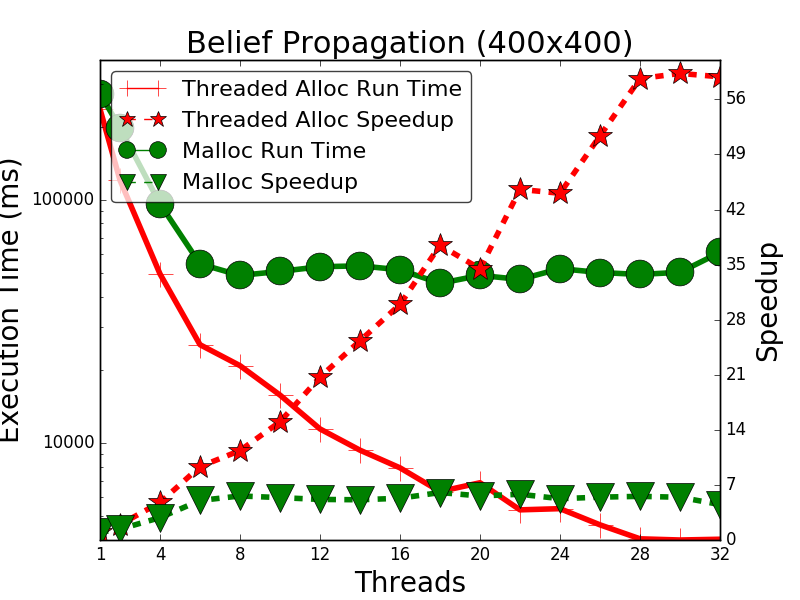
\includegraphics[width=\textwidth]{experiments/scalability/malloc-allocator-belief-propagation-400.png}
                \label{fig:implementation:malloc_bp}
        \end{subfigure}
        ~
        \begin{subfigure}[b]{\smallplotsize\textwidth}
                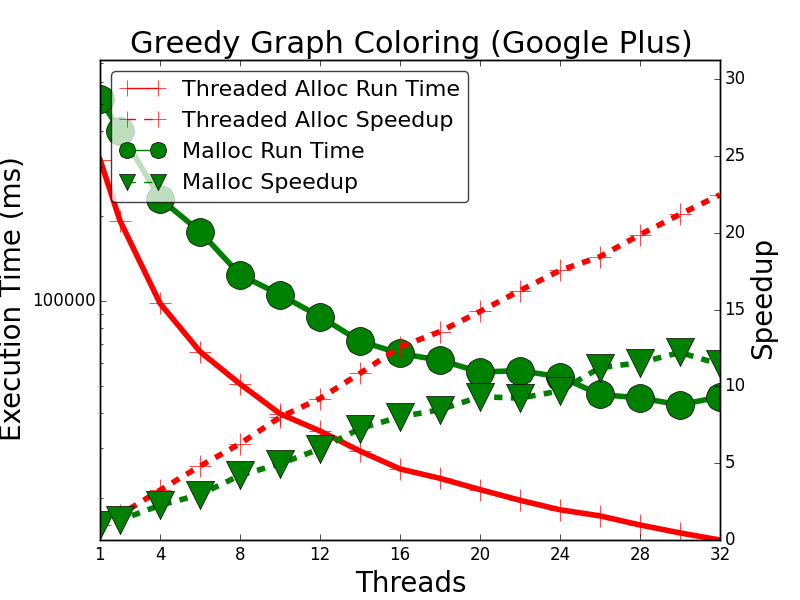
\includegraphics[width=\textwidth]{experiments/scalability/malloc-allocator-greedy-graph-coloring-gplus.png}
                \label{fig:implementation:malloc_ggc}
        \end{subfigure}
        ~
        \begin{subfigure}[b]{\smallplotsize\textwidth}
                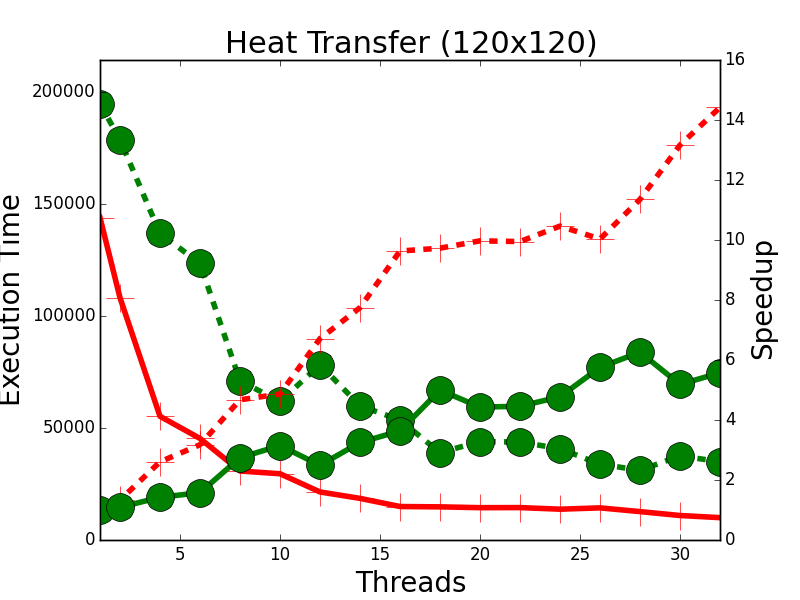
\includegraphics[width=\textwidth]{experiments/scalability/malloc-allocator-new-heat-transfer-120.png}
                \label{fig:implementation:malloc_ht}
        \end{subfigure}
        ~
        \begin{subfigure}[b]{\smallplotsize\textwidth}
                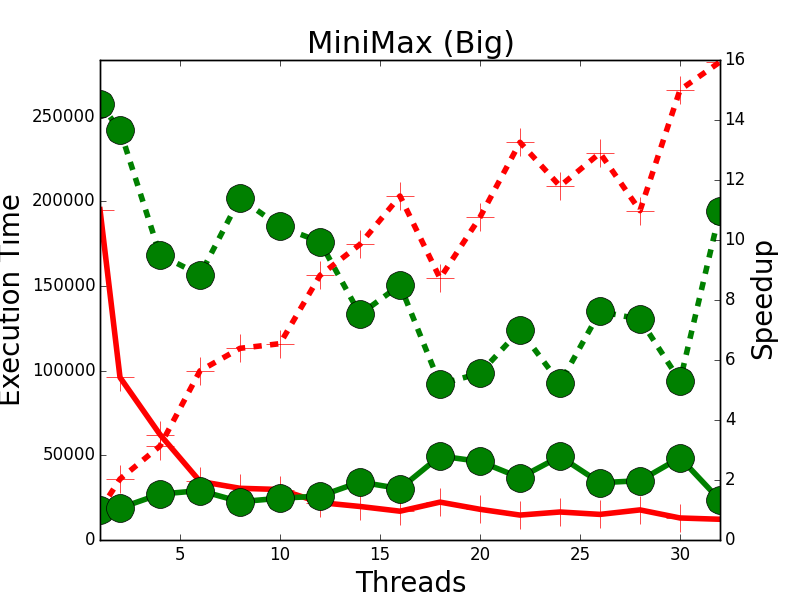
\includegraphics[width=\textwidth]{experiments/scalability/malloc-allocator-min-max-tictactoe-big.png}
                \label{fig:implementation:malloc_minimax}
        \end{subfigure}
        ~
        \begin{subfigure}[b]{\smallplotsize\textwidth}
                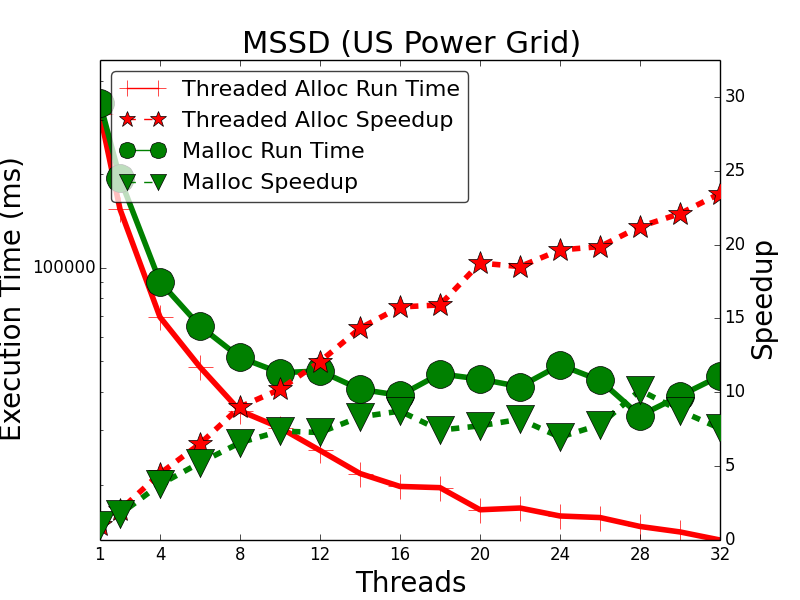
\includegraphics[width=\textwidth]{experiments/scalability/malloc-allocator-shortest-uspowergrid.png}
                \label{fig:implementation:malloc_sssp}
        \end{subfigure}
        ~
        \begin{subfigure}[b]{\smallplotsize\textwidth}
                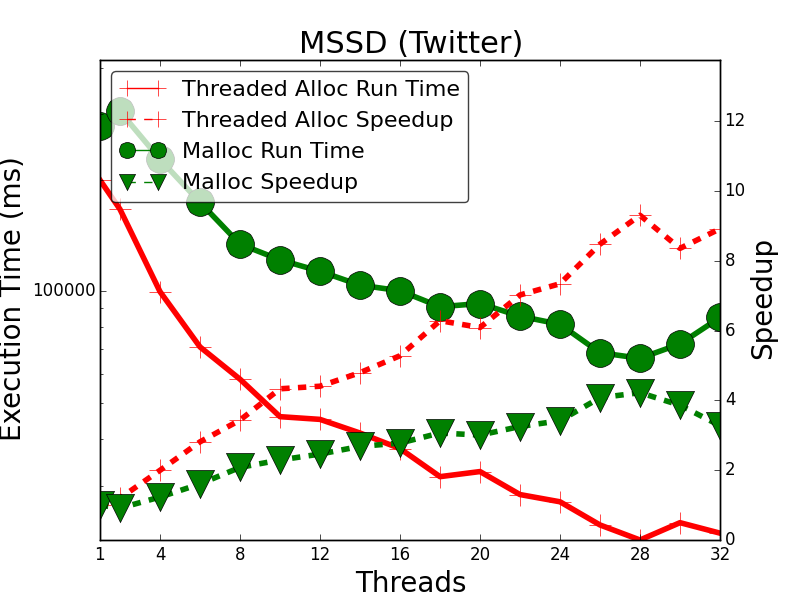
\includegraphics[width=\textwidth]{experiments/scalability/malloc-allocator-shortest-twitter.png}
                \label{fig:implementation:malloc_sssp}
        \end{subfigure}\\
        \begin{subfigure}[b]{\smallplotsize\textwidth}
                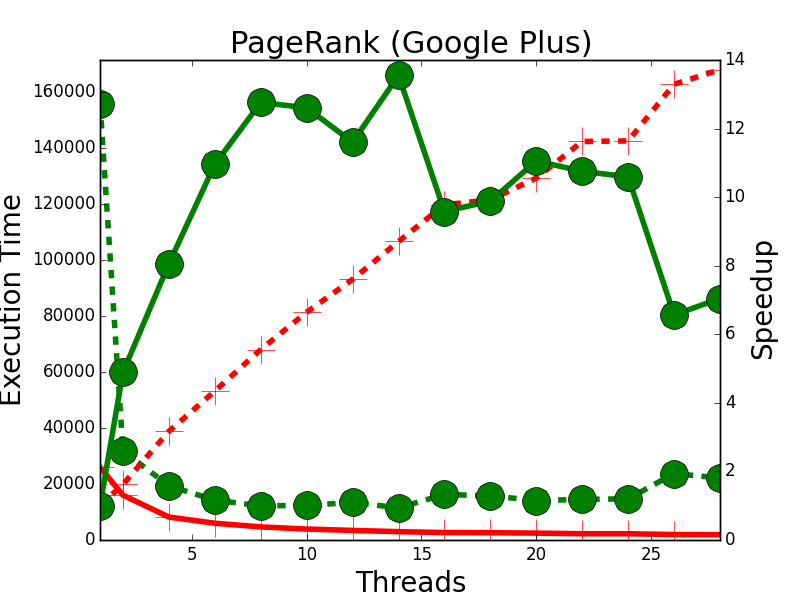
\includegraphics[width=\textwidth]{experiments/scalability/malloc-allocator-pagerank-gplus.png}
                \label{fig:implementation:malloc_pagerank}
        \end{subfigure}
        ~
        \begin{subfigure}[b]{\smallplotsize\textwidth}
                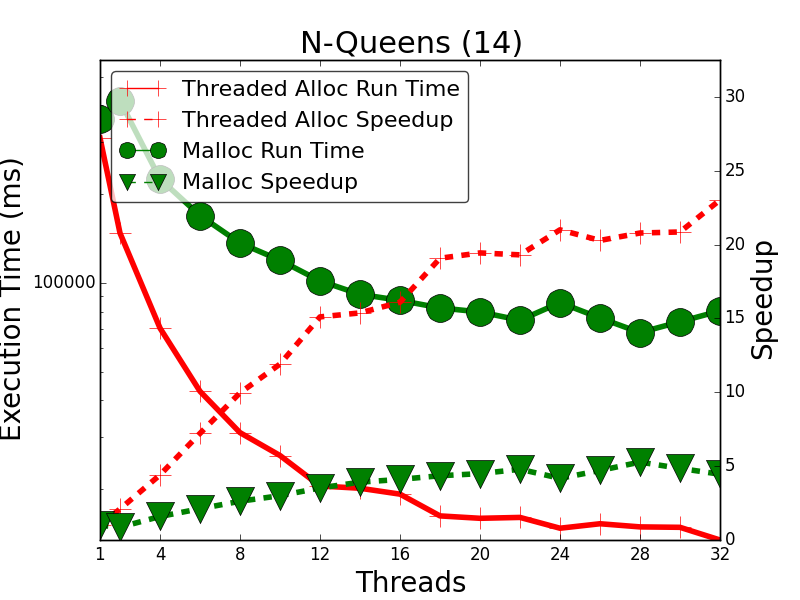
\includegraphics[width=\textwidth]{experiments/scalability/malloc-allocator-8queens-14.png}
                \label{fig:implementation:malloc_queens}
        \end{subfigure} \\

        \caption{Comparing the threaded allocator described in
           Section~\ref{section:implementation:allocation} against the
           \texttt{malloc} allocator provided by the C library. The threaded
           allocator is represented by plus markers, while \texttt{malloc} is
        represented by circular markers. Note that the two speedup lines (right
     axis) use dashed lines, while the two lines representing the run time (left
  axis) are contiguous.}

        \label{fig:implementation:malloc_results}
\end{figure}
